%================================================================
\chapter{Analysis Activities}
\label{ch:analysis-activities}
%================================================================

%--------------------------------------------
\section{A single year of vital statistics}
%--------------------------------------------

A problem most people can relate to is demography. Millions of people are born in the US every year. Recording birth events is necessary for legal matters such as obtaining a driver's license or other forms of government-issued identification. However, recording, keeping, and using this information has challenges that exemplify many aspects of data analysis, as this exercise will demonstrate.

\begin{warningbox}[title=DO NOT USE ANY FORM OF AI HERE]
There is a reason for the request not to use AI for the analysis tasks, e.g. LLMs. \textbf{DO NOT DO IT}. If you do it, you will lose an essential component of training. During the workshop, we will discuss how to solve the problems in this section and more advanced problems with AI. We will explain the rationale for this request within the first hour of the in-person workshop.
\end{warningbox}



Since 1969, all births recorded in the US are available as digital records from the National Center for Health Statistics (NCHS) from the Centers for Disease Control and Prevention (CDC). Only between 1969 and 1988 the date and time of birth is publicly available; starting on 1989, only the week of birth is recorded. Why is the date and time of birth no longer recorded? \QA


The NCHS keeps records of place of birth, assistance during delivery (at home, with doctors, with midwives), level of education of the parents, place of residence, weight at birth, number of weeks of gestation, number of siblings, birth order, etc. In total, over 100 variables are recorded.

I have made available two files for you: a compressed file with birth records from 1969, and a data dictionary. The uncompressed data file is about 380 MB in size. The data is contained in a "flat file". This means that every line of text in this file is a continuous chain of characters. We must extract information from this type of files with a "dictionary" that tells us the beginning and ending columns of a given variable. Why was this format used? \QA


Please answer the following questions:
\begin{enumerate}
	\item How many live births occurred in Texas in 1969 from mothers residing in Texas?	\QA
	\begin{itemize}
		\item Bonus question: How would you visualize births from each state with respect to every other state?
	\end{itemize}
	\item Show graphically how the level of education of the mother is related to the birth order (1st born, second child, third, etc.)	 \QA
	\begin{itemize}
		\item Bonus question: How would you visualize each variable with respect to every other variable?
	\end{itemize}
\end{enumerate}

It is possible that you might not know how to answer some of these questions on first contact with this problem.

A simple program that can help you explore this file is

\begin{lstlisting}[language=Python]
f = open("US1969.dat", "r", encoding="cp1252")
counter = 0;
for x in f:
    if x[0] == "9" and [... other conditions?]
        counter = counter + 1
print(counter)
\end{lstlisting}
%

Note that in Python indexing is subtle. For example:

\begin{lstlisting}[language=Python]
x = [10, 20, 30, 40, 50]
x[1:3]  # This is [20, 30]  (indices 1 and 2, not 3)
\end{lstlisting}

The instruction \textit{encoding=``cp1252"} is necessary in non-Windows systems due the presence of single-byte character encoding of the Latin alphabet, used by default in the legacy components of Microsoft Windows for English and many European languages including Spanish, French, and German. If you remove this instruction, the following error might show up in non-Windows operating systems: ``'utf-8' codec can't decode byte...''

A common approach to extract information from flat files is by importing it into Excel. The ``\textit{Text Import Wizard}'' (typically shown as in Figure \ref{fig:Excel}) would guide you through the process of identifying variables by column. However, this results in a problem. Describe it. \QA

\begin{figure}[hb]
	\centering
		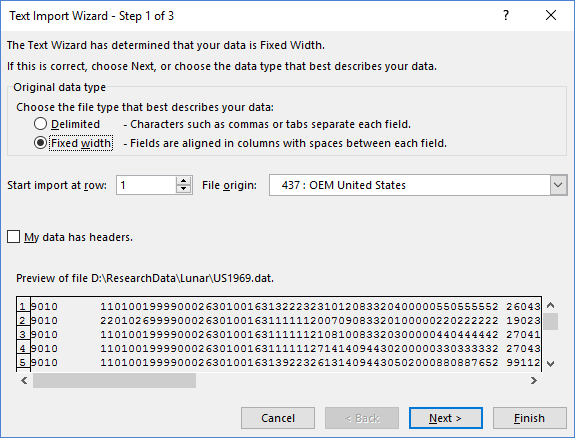
\includegraphics{../images/Excel.png}
	\caption{Excel's Import Wizard}
	\label{fig:Excel}
\end{figure}

